
\documentclass[11pt]{article}

\usepackage{geometry}
\geometry{a4paper,margin=3cm}


\usepackage{graphicx}
\usepackage{float}
\usepackage{enumitem}
\usepackage{cite}
\usepackage{natbib}
\usepackage[T1]{fontenc}
\usepackage[titledoc]{appendix}

\usepackage{pdfpages}

\DeclareGraphicsExtensions{.pdf,.png,.jpg,.jpeg,.ps}



\begin{document}

\title{Signal Green Final Report}

\author{Waqar Aziz, James Kerr, Adeela Saalim, Andrea Senf, Yoann Strigini}

\maketitle 

\newpage



%\listoftables


\tableofcontents
\addcontentsline{toc}




\newpage


\section{INTRODUCTION}


This work was first and foremost an opportunity for working in a group. Employers want engineers who are not only skilled in their craft, but also persons who are able to collaborate, work well as part of a team, and invest in project aims and those working to achieve them. Our team was able to develop a simulation that involved each member in the process. In spite of differing abilities and communication styles, each person was able to contribute in important ways. Together we accomplished much more than any one of us could have created on our own in the time provided.

The software engineering part of this project focused on creating a traffic simulation software where we can test various traffic management strategies. We wanted to create a simulation that would be visually interesting with user modifiable variables and that would have potential for further expansion and use.

We were able to create a simulation that is interesting, flexible, and allows different layouts and road policies to be tested and visually represented. Any geographic information system (GIS) map shapefile representing road networks can be loaded into our simulator and could easily be extended to take into account any other relevant attributes.

Our team further gained a more practical understanding of agent based modelling (ABM) through using Repast Simphony, and gained experience with version control through using GitHub.



\section{BACKGROUND}

\subsection{Traffic Flow Forecasts}

Analysis of complex urban networks and traffic flow models is the groundwork for reliable traffic flow forecasts, which are widely used to avoid traffic congestion and maximise road network capability in metropolitan areas.[11k] Predictions of traffic growth published by the UK Department of Transport in 2013 show that despite a slowdown in the past decade mainly due to economic recession and high oil prices, traffic on all roads in England are expected to grow by about 45\% by 2040 \cite{10j}. (See Figure 1.)

\begin{figure}[h]
\begin{center}
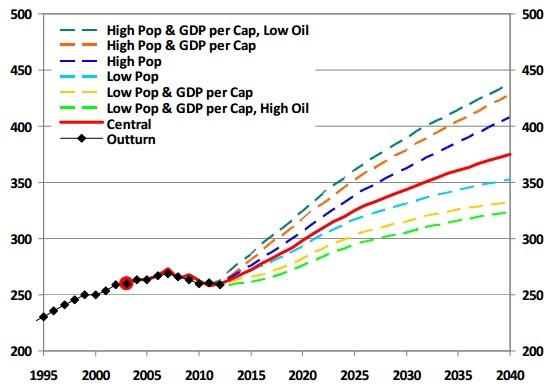
\includegraphics[scale=0.7]{england_traffic}
\caption{England traffic growth}
\end{center}
\end{figure}


Consequently, causes and effects of traffic congestion have been studied extensively in order to face the increasing road network saturation. Several factors that have significant impact on traffic flow have been identified, including the following: 
\begin{singlespace}
\begin{itemize}\itemsep0pt
\item Road/Traffic policy approaches
\item Timing and cost of journeys
\item Types of vehicles and speed
\item Junctions and bottlenecks
\item Lane splitting and joining
\item High occupancy vehicle lanes
\item Driver\textquoteright s behaviour
\item Rush hours
\item Occasional factors such as car accidents, road works or bad weather
\end{itemize}
\end{singlespace}


The model we implemented has been designed with acceptable trade-off between accuracy and computational complexity. We have therefore selected the following set of urban traffic factors:
\begin{itemize}\itemsep0pt
\item Different types of vehicles, e.g. trucks are slower than cars and are less likely to overtake
\item Driver\textquoteright s behaviour, e.g. reckless drivers do not stop at amber signal
\item Journey of vehicles is based on best route according to roads\textquoteright length and speed limit
\item Roads can have multiple lanes, fast vehicles try to overtake slow ones
\item Different traffic management policies, including traffic lights and/or give way signs
\end{itemize}

The ultimate goal of traffic simulation is to create space for people to move along their journeys in a safe manner with consistent progress. Data extracted from simulations will be evaluated later in this report to demonstrate that our simulation is useful for developing practical policies for the future.



\subsection{Selected Bibliography}

Our team began by researching various traffic simulation models and code available online. Some of the more significant included the following:

The entire team went through a very good tutorial to learn Simphony basics [Collier and North\cite{7g}]. This tutorial was an excellent introduction to Simphony and had clear parallels to our simulation. 

Macal and North\cite{5e} offered an important document that argues that \textquotedblleft only agent-based models can explicitly incorporate the complexity arising from individual behaviors and interactions that exist in the real-world. \textquotedblright [1458] It further shows the wide uses of Repast in various fields\cite{5e} [1457 Table 1]. The article notes that agent modelling using desktop environments like Repast Simphony is a good way to explore the potential of ABM in a brief space of time and with minimal training investment \cite{5e}[1464] and this is a benefit our team hoped to gain through this project. 

One excellent resource [Lansdowne\cite{4d}] offered a detailed example of an agent-based traffic simulation; referenced for approach and features often considered when creating an agent based model. This was well written and fairly comprehensive. 

Team programmers referenced Lee\textquoteright s\cite{8h} work for coding lane changing and gap acceptance logic. Benhamza et al\cite{6f} also provided many ideas regarding behaviour rules that was useful, as was the brief but descriptive discussion of modelling. 

Early documents team members considered included Wagner\cite{1a} simulation, which gave us a picture of what an interesting simulation and its code might look like, and Malleson and Addis\cite{3c} demonstrated one way to conceptualize moving cars along a road from origin to destination. [Note: This link has since been removed.] 

Shiffman \cite{2b} offered a very good piece on what coding with cellular automata involves for those on the team unfamiliar with the concept. In the early stages of the project we thought coding using cellular automata might be an approach we would utilize; this was later decided against in favour of ABM. 



\section{REQUIREMENTS AND DESIGN}


Our traffic simulator is an agent-based, non-deterministic, discrete-time simulator for microscopic traffic modelling which allows different traffic policies on user-defined Geographic Information System (GIS) maps to be tested. 

An Agent-Based modelling (ABM) simulation seemed most appropriate for a traffic simulation\cite{5e} [see 1465]. ABM uses entities (agents) to embed certain behaviours and they exist in a certain environment. Agents are autonomous, have objectives and goals, and can interact with other agents. ABM is particularly suitable for traffic simulation because agents, such as vehicles and traffic lights, can adapt to the evolving environment and accommodate changes, e.g. a vehicle needs to accelerate when a traffic light turns green.

The system is non-deterministic, with future states of traffic flow depending on unpredictable events, just as real-life traffic phenomena always have a degree of unpredictability. Randomness is added by the use of a random seed which changes during each run: with same input, output is always different. 

A discrete time model, given its iterative nature, is convenient for traffic simulations. Every tick the current state of the agents is evaluated, algorithms are recomputed, and the overall state of the system is updated. For example, traffic lights change light every n ticks, and each vehicle\textquoteright s velocity is updated accordingly. Our simulation updates state every tick of the clock.

Microscopic traffic models typically simulate the behaviour of single vehicles using microscopic properties such as the vehicle\textquoteright s position and velocity. Our simulation uses the following common decision models\cite{8h}: Car-following model, Lane-selection model, and Gap-acceptance model.

Lastly, GIS integration allows real maps to be loaded into the system. GIS is the de-facto standard for most professional traffic simulators, and governments regularly publish GIS maps about road networks, which are freely available for download. Virtually any GIS map can be loaded into our system.

\subsection{Functional Requirements}

We set out the following functional requirements:

\begin{itemize}\itemsep0pt
\item \textbf{FR1: Maps} 
	\begin{itemize}
	\item FR1.1: Multiple maps can be used
	\item FR1.2: Use GIS standard
	\end{itemize}
\item \textbf{FR2: Roads}
	\begin{itemize}
	\item FR2.1: Can have multiple lanes
	\item FR2.2: Traffic flows bi-directionally 
	\item FR2.3: Vehicles appear to run along roads
	\item FR2.4: Vehicle follow speed limits of road
	\end{itemize}
\item \textbf{FR3: Vehicles}
	\begin{itemize}
	\item FR3.1: Variable number of vehicles 
	\item FR3.2: Accelerate and decelerate
	\item FR3.3: Appear visually different by type
	\item FR3.4: Type car with unique behaviour
	\item FR3.5: Type truck with unique behaviour
	\item FR3.6: Exhibit passing behaviours
	\item FR3.7: Journey calculated by road length and speed limit
	\end{itemize}
\item \textbf{FR4: Junctions}
	\begin{itemize}
	\item FR4.1: Connect roads
	\item FR4.2: Type give way
	\item FR4.3: Type signal
	\item FR4.4: Type roundabout
	\item FR4.5: Signals change between red, green
	\item FR4.6: Signals supports orange
	\item FR4.7: Vehicles stop at red and go at green
	\item FR4.8: Source at junctions
	\item FR4.9: Stop/wait before special junctions
	\end{itemize}
\item \textbf{FR5: Simulation}
	\begin{itemize}
	\item FR5.1: User controlled variables
	\item FR5.2: Show statistics report feature
	\item FR5.3: Runs on different machines
	\end{itemize}
\end{itemize}

Functional requirements are divided into High Priority, Low Priority, and Optional Requirements, and were released iteratively.
\\ \\
High Priority (SG V1.0): FR1.2, FR2.2, FR2.3, FR3.1, FR3.7, FR4.1, FR4.2, FR4.5, FR 4.7, FR4.8, FR4.9, FR5.2
\\ \\
Low Priority (SG V2.0): FR2.1, FR3.2, FR3.3, FR3.4, FR3.5, FR3.6, FR4.3, FR4.4
\\ \\
Optional (SG V3.0): FR1.1, FR2.4, FR4.6, FR5.1, FR5.3

\subsection{Milestones}

For the purposes of planning, our team set Milestones to measure what we wanted to accomplish. This were our requirements as they stood at the beginning of February: 
\\
Milestone 1 (Required):
%\begin{itemize}\itemsep0pt
\begin{itemize}
\item deadline: 23 February  \item code compiles and runs simple simulation \item vehicles run on a map  \item variable number of vehicles \item vehicles make decisions to reach a goal
\end{itemize}
\\
Milestone 2 (Required):
\begin{itemize}\itemsep0pt
\item deadline: 8 March
\item implement basic vehicle type: car
\item traffic flows bi-directionally
\item junctions
\item signals, give way, roundabouts
\item multiple maps in GIS standard
\item cars have different behaviours: timid, aggressive, patient
\item multiple lanes on some roads
\end{itemize}
\\
Milestone 3 (Optional):
\begin{itemize}\itemsep0pt
\item deadline: 16 March
\item vehicles appear visually different by some criteria (type/behaviour, speed, congestion)
\item speed limits on roads
\item implement vehicle types: lorry, emergency, motorcycles
\item vehicles exhibit passing behaviours
\end{itemize}
\\
Possible Traffic Policy Implementations for Simulation:
\begin{itemize}\itemsep0pt
\item all light junctions
\item all roundabout/give way junctions
\item mix lights/roundabout junctions
\item variable speed limits
\item same junction policy with varying levels of congestion
\end{itemize}
\\

\subsection{Language and Framework}

The team began by choosing a programming language for development. We quickly settled on Java as our language, as everyone on the team was familiar with it and Java is commonly used in industry. Java is fast enough to simulate hundreds of agents, is entirely object oriented which makes it ideal for an agent paradigm, and currently the most popular Agent Based Modelling framework is in Java. C++ was considered, but the team preferred Java for its ease of coding. A scripting language like python would have enabled fast development, but team members were unfamiliar with it, it is computationally slow, and so not a good choice for modelling with many objects.

For a framework we considered several options. We could code an entire agent based traffic simulation ourselves; this was not selected due to the enormous coding task this would involve, and we were concerned we would not meet all the requirements for the assignment in the time allocated. We considered NetLogo, but decided it did too much work for us; we would do almost no coding ourselves, and very little logic to create. We wanted to show our own ability to code and create our own logic.



\subsection{Repast Simphony}

We settled on Repast Simphony, a general application programming interface (API) providing us tools, libraries, and plug-ins to create a simulation while allowing us to code and implement appropriate logic for the desired simulation. Repast comes with a BSD software license and is widely used in many fields of academia.\cite{5e} [table 1, 1457] Repast Simphony provided the following benefits that made it a good fit for our group project:

\begin{itemize}\itemsep0pt
\item As a framework for Java, it is fully object oriented and everything is created as a Plain Old Java Object. It includes Java libraries and .jar utilities, and all objects are rewritable.
\item It provides an ABM environment with a practical skeleton of agents and their contexts, and includes features such as behaviour activation, a discrete event scheduler and Watcher component, and space and grid management.
\item It provides a flexible plug-in framework, allowing the developers to use, modify, or write plug-ins. It provides the ability to integrate advanced elements into our code such as importing GIS maps, multi-threading, XML configuration files, and other advanced features.
\item It includes charting and data collection functions, so we can focus on deciding on traffic policies and changing these parameters rather than spending time finding ways to display and record the results. The probe function is particularly useful for ABM testing.
\item It provides an attractive display graphical user interface (GUI) we can modify to suit our needs and make a more interesting simulation, including user defined options at runtime and 2D and 3D visualisation and GIS plugins. One can create new or rewrite existing plug-ins if one wishes.
\end {itemize}

The benefits of Simphony come at the flipside cost of there being more opportunities for our team to display skill in modelling concepts and logic rather than a mastery of Java programming skill. When our team chose ABM as our design platform this meant behaviour and goals became more central than designing passive functions \cite{4d}, and we trust our ability to create an interesting system shows in our project and does credit to our ability. The team spent some time learning the framework, but this was considered a good investment for the benefits.

\\ 

\section{Implementation}

\subsection{Simphony and Our Code}

The integrated development environment (IDE) for Simphony is a preconfigured Eclipse IDE. Eclipse Simphony varies from the normal Eclipse IDE in that it contains custom views, run configurations, and it adds three .jar files to the buildpath: JOGL (Java bindings for openGL), Java3D, and JAI (Java Advanced Imaging). These .jar files are used to create graphical representation of objects. Simphony also requires a ContextBuilder to initialize and drive the simulation, replacing the Java Main() run method; in our code class SignalGreenBuilder.java implements the ContextBuilder for the program.

While Simphony provided a very useful API, our team determined how each agent and behaviour should be modelled and the logic used to describe each object. For example, Simphony had no effect on how we modelled traffic signals. There is no agent superclass, no inheritance interfaces, no exposed code provided. The actual creation of agents and the method of that creation is the work of the programmers. 

Simphony provided nice helper features and many tools to increase the speed at which we could code. Our code uses its background foundation required for ABM, including multi-threading, the Clock/Watcher, having objects automatically drawn on the screen, and agents being aware of their environment. While our team wanted to especially take advantage of Simphony\textquoteright s visualisation benefits, our core requirements are based around the logic of the agents, not their appearance.



\subsection{GIS maps}

Geographic Information System (GIS) maps capture geographical data from the real world and saves this data in standardised shapefiles (.shp). By using GIS maps our simulation can use maps and physical data from every country on the Earth \cite{12m}. 

Shapefiles store the geometry of the road networks along with attributes such as road name, speed limits, etc. These are accessible through the UI so one can see pertinent information (eg. which road is experiencing congestion) while running a simulation. 

Using GIS files gives our simulation the relevance of being able to run various policies on actual existing roads. Our simulation is easily extensible to include other factors relevant to particular roads that our simulation does not handle. Adding additional road features will enable full utilisation of the GIS maps.

GIS overhead makes up a significant portion of our codebase. The shapefile is loaded in the constructor using a static path plus user input for the specific file. 

Every vehicle instance has two sets of coordinates: realPos for the UI, and networkPos for calculations. There are calculations required for converting between the polar and grid north coordinates. 

Method Utils.distance - uses geoditic calculator to get distance in metres between two GIS coordinates. This uses the external library geotools.

Vehicle.moveTowards - takes in a coordinate and distance, converts it ot GIS coordinates, and updates positions in the real GIS geography as well as the UI.

getPosition - takes a single coordinate and returns an array of perpendicular coordinates, two logical and two real.

getNetworkPosFromRealPos and getRealPosFromNetworkPos both wrap the method getPosition, and based on the vehicles' current lane returns a coordinate from the array.

getPosition further calls two methods in Utils: getAzimuth and createCoordsFromAngle.

Utils.getAzimuth - takkes in two coordinates and geography, returning the azimuth as a double. This is very complex and so uses the geodetic calculator found in the extrenal libraary geotools.

utils.createCoordsFromCoordAndAngle - This meethod requires the azimuth angle, coordinate, distance, and geograhy. the azimuth is converted to radians to make the calculations easier, and then based on whether the angle is +90 or -90 degrees adjusts it to place it in one of the four quadrants. The two angles are then converted into degrees.


\subsection{Agents and Environment}


The architecture for our simulation engine is a hierarchy of Java classes, where each class is either an agent or an environment. Agents are objects that exhibit behaviours and can either be of fixed geography (eg: junction, road) or they can move on the GIS projection (eg: vehicles and their subclasses). Agent behaviour can be embedded through the agents reacting to the environment themselves, by using the watcher component which listens for events and triggers actions, or by globally scheduling events to happen.

An environment forms a container for agents and includes the Road Network Topology (the network), and GIS Geography (the geography). The environment is coded in continuous space with (X,Y) coordinates on a directed graph network, with the Network being the topological relationship between each road segment. At any time each agent knows its position on the Geography; vehicle agents can ask the Network for their route and then follow this course along each road segment. Continuous space also allows the user interface to display agents in detail during the simulation.

Repast offers a ContextBuilder component containing a framework for creating agents and environments. The team used the framework to model entities and features including (but not limited to): vehicles, roads, junctions, road network topology, and GIS geography. We also coded all behaviour logic (direction, volition, velocity, etc) for the agents.

We used Styled Layer Descriptor (SDL) files to create the presentation; SDL is an extension of OpenGIS which is open source and provides the benefit of XML format.


\subsubsection{The SignalGreenBuilder Class}


Class SignalGreenBuilder.java builds the road network and the GIS geography for our simulation and initialises the agents. It is the only ContextBuilder class for the program. At the highest level of abstraction, the program Context contains a graph (Road Network) of vertices (Junctions) connected by paths (edges). The Road Network is a directed graph representing the road topology, and the GIS geography is used to display the simulation. 

Repast has built-in GIS integration, so reading in spatial data is done by iterating over each Feature object of the ShapefileDataStore file (shapefile). Every feature of type \textquotedblleft MultiLaneString\textquotedblright represents a road object with its spatial location and other attributes. Creating a road network is achieved by linking edges together, and the road network topology is built with pairs of connecting junctions.

Any GIS map shapefile (.shp) representing road networks can be loaded into our simulator. The simulator uses some GIS attributes for modelling vehicle\textquoteright s behaviour (ex. road type, max speed, etc.) and could easily be extended to take into account any other relevant attribute.
GIS maps were simplified by removing the road coordinates between the Junctions to make it more efficient; creating road agents with only the endpoint coordinates specified prevents very complex urban street maps from becoming too computationally expensive. (See Figure 2.)
\\

\begin{figure}[H]
\begin{center}
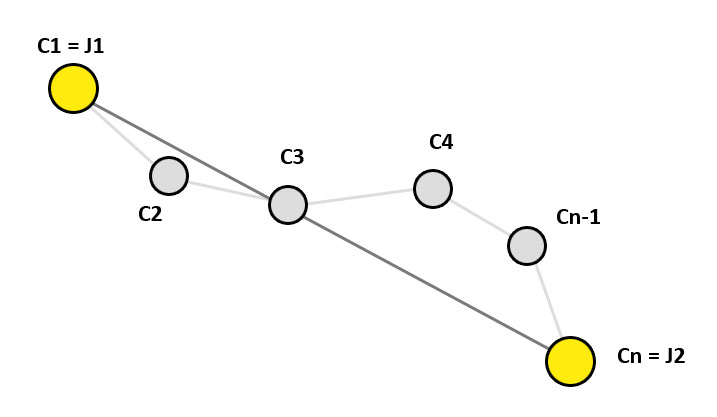
\includegraphics[scale=0.4]{creating_road_segments_from_shapefile}
\caption{creating road segments using only endpoints}
\end{center}
\end{figure}

\\
Each Road agent is added to both the Context and the GIS geography, along with two Lane agents for each side of the Road (used only for displaying vehicle graphics on the UI). A Repast edge is then added to the road network, and the Repast edges are then linked together to create the road network topology. This is done by keeping a cache of all previously created Junctions, so every time a new Road agent is created the cache is checked to see if there already exists Junctions for its end point coordinates. If there is, then we know all roads linked to those Junctions are also linked to the Road agent being created, and we do not need to create any more new Junctions. see \cite{3c} for more detail. 
\\

\begin{figure}[H]
\begin{center}
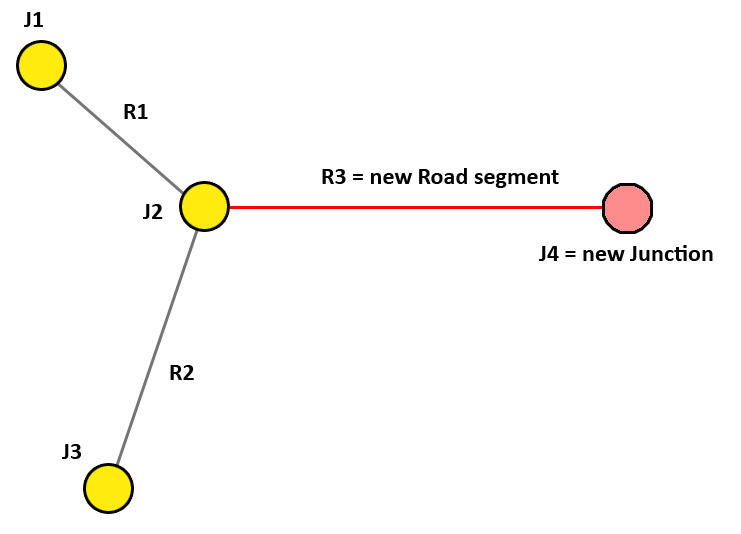
\includegraphics[scale=0.3]{creating_new_roads}
\caption{Creating new roads}
\end{center}
\end{figure}

\\
As an example, consider Figure 3.

Before R3 is added:
Cache of Junctions = (J1, J2, J3)
Road network = (R1, R2)
Road network topology = (<J1, J2>, <J2, J3>)

After R3 is added:
Cache of Junctions = (J1, J2, J3, J4)
Road network = (R1, R2, R3)
Road network topology = (<J1, J2>, <J2, J3>, <J2, J4>)

Once the whole shapefile has been read, the GIS geography is displayed on the UI, as shown on (see Figure 4). In this example we have loaded a map of the main avenues of New York City and clicked on a Road agent to show its attributes: name = Madison Av, speedLimit = 65 Km/h, length = 4,805 meters. Virtually any urban street map can be loaded into Signal Green.
\\

\begin{figure}[h]
\begin{center}
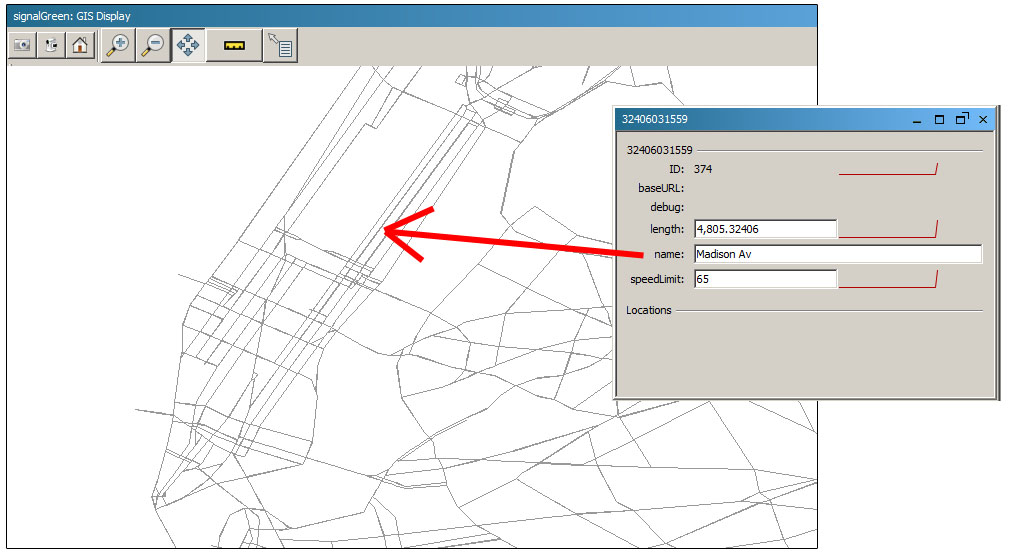
\includegraphics[scale=0.4]{GIS_display_manhattan_loaded}
\caption{Manhattan in our simulator}
\end{center}
\end{figure}
\\

\subsection{The Vehicle Class}


Class Vehicle.java is a very important class which initializes vehicles, assigns vehicles their individual behaviour, type, source, and interactions, and contains the generic vehicle constructor. Classes CarVehicle.java and TruckVehicle.java extend the Vehicle.java class and override the constructor to create three new types of vehicles: slow cars, fast cars, and trucks. Each type has its own adjusted maxVelocity and visual icon. 

Method initVehicle() creates a type of vehicle agent and assigns it a random source and destination junction that includes the vehicle\textquoteright s route to that destination. For performance reasons we did not find it feasible to calculate the best path at each vertex; instead the entire path is chosen at initialisation using the highly optimised shortest path algorithm provided by Repast Simphony. The path is shortened as each junction is reached on the way to the destination. When the destination is reached, new random values are chosen and the process repeats.

Method computeDisplacement() is used to determine exactly how far in metres the vehicle should travel based on the vehicle\textquoteright s attributes. 


\subsubsection{Method Step()}


A vehicle\textquoteright s vision is the distance around which a vehicle is aware of its environment and is calculated based on constant values DIST{\_}VEHICLES and DIST{\_}VEHICLES{\_}STOPPED. Method step() determines individual vehicle behaviours, including interaction with junctions and other vehicles, increasing/decreasing speed, changing lanes, and moving the vehicle along the map.

The vehicle checks the speed and distance of any vehicles in its path, slowing if needed to an optimal velocity. If a vehicle observes a slower moving vehicle in its path, it makes a decision whether or not to change lanes. The vehicle also checks for approaching junctions, decelerating to a stopped position before the light if a red light is in view. If no other vehicles or junctions are in its vision it will accelerate to its maxVelocity (see Figure 5).
\\

\begin{figure}[H]
\begin{center}
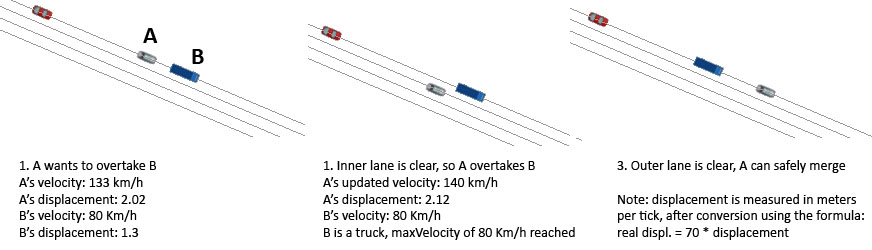
\includegraphics[scale=0.4]{overtaking}
\caption{Faster vehicle overtakes slower truck}
\end{center}
\end{figure}

\\
The method step() works as follows. (See diagram in Figure 6.) Assume the current vehicle V is heading towards a junction J[i]. J[i] is the next node on its route, J[1..n], where n is the number of nodes, J[1] and J[n] are V\textquoteright s origin and destination. 

V needs to first decide which lane it wants to go to (lane selection decision model, step 1.2) and check that the road is clear (gap acceptance decision model, step 2). 

In steps 3 and 4, V tries to either accelerate or slow down, depending on the outcome of the previous steps. 

Next, if V is close enough to J[i], traffic management policies are evaluated (step 8): for example, if J[i] uses traffic jams, then V asks J[i] if it has to wait (Light.RED signal detected, step 8.1.1). Finally, displacement is executed, meaning V\textquoteright s position is updated both in the road network topology and in the GIS projection (step 9).

V checks what is the J[i] on the route J[n]. It knows which vehicles are approaching because it holds a priority queue of incoming Vehicles for each road segment, where weights are the distance from V to J[i]. This is an efficient solution as insertion is done in O(log n), while removal is done in constant time.
\\

\begin{figure}
\begin{center}
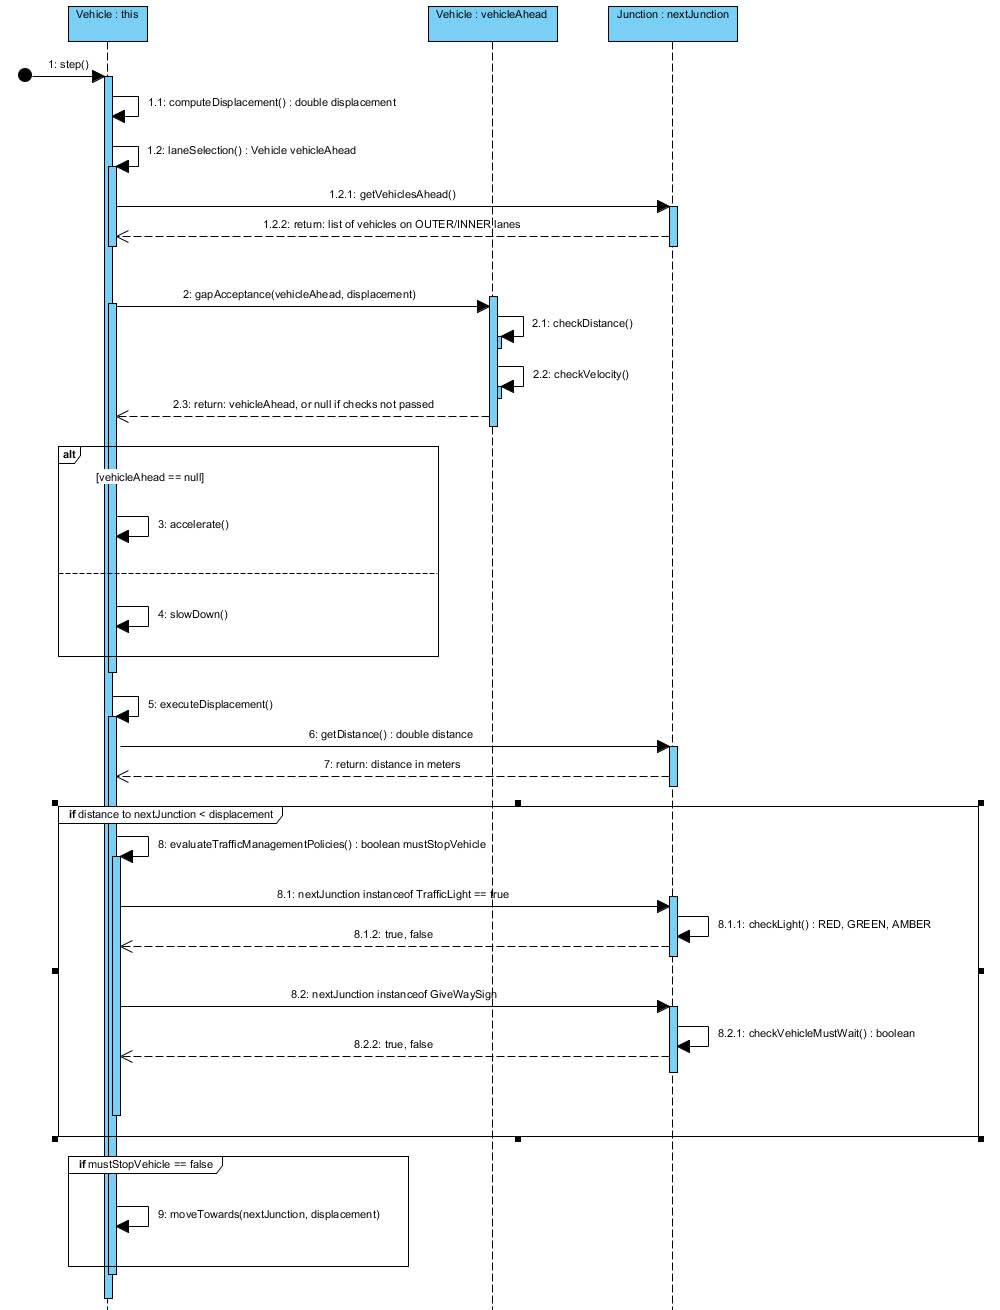
\includegraphics[scale=0.45]{step_method_seq_diagram}
\caption{Sequence diagram for step() method}
\end{center}
\end{figure}

\\
From Repast\textquoteright s point of view, Step() method is executed every iteration of the simulation, using the Java annotation: @ScheduledMethod(start = 1, interval = 1) meaning that it starts from tick one, and gets executed every tick.


\subsubsection{Simulation Calibration}

Manual testing of SG was fundamental for proper calibration of simulation parameters.
Improper calibration leads to invalid output, thus special care must be taken when adjusting values to make the simulation visually realistic. The Constant class holds all arbitrary calibration parameters.

Simulation parameters and relevant measures are summarised as follows:
\begin{itemize}
\item 1 simulation tick = 1 second
\item GIS projection distances reflect real distances, and are measured in meters
\item Minimum distance between vehicles to avoid collisions = 1.8 meters
\item Arbitrary acceleration factor of vehicles = 1.6
\item Real vehicle displacement in meters = displacement * 70
\item Displacement equation: x = v0 * t + 1/2 a * t * t, where x is the displacement, v0 the initial velocity, a the acceleration, t the time – which is arbitrarily set to 4.
\item Truck maximum speed = 80 Km/h
\end{itemize}



\subsubsection{Moving on GIS Geography}


GIS maps use an azimuth angle system to map coordinates on to spherical maps of the Earth. These allow for more accurate and realistic simulations, where the topology and actual distances in metres are true, and the maps are based on true North. Using GIS maps adds a layer of complexity to our code, as the UI uses a flat Cartesian system with simple (X,Y) coordinates and is based on grid north. So our simulation needs to translate GIS data for the UI.



The vehicle.java class determines the behaviour of vehicles so they follow roads. This required special coding, as GIS images point true north and use azimuth coordinates for its 3D mapping, while the UI points to grid north and uses simple (X,Y) coordinates for the grid. 

Azimuth coordinates allow one to measure distances and plot locations in a spherical coordinate system, and our code utilized this form of measurement in moving the vehicles along the maps. We referenced \cite{9i} to see how one could compute the correct angle for displaying graphics on the UI. 

This further required the use of kinematics equations for plotting the direction of vehicles in several methods. Kinematics is the study of objects moving through space. Because we used GIS maps, all calculations along the map involve real distances.
\\

\begin{figure}[H]
\begin{center}
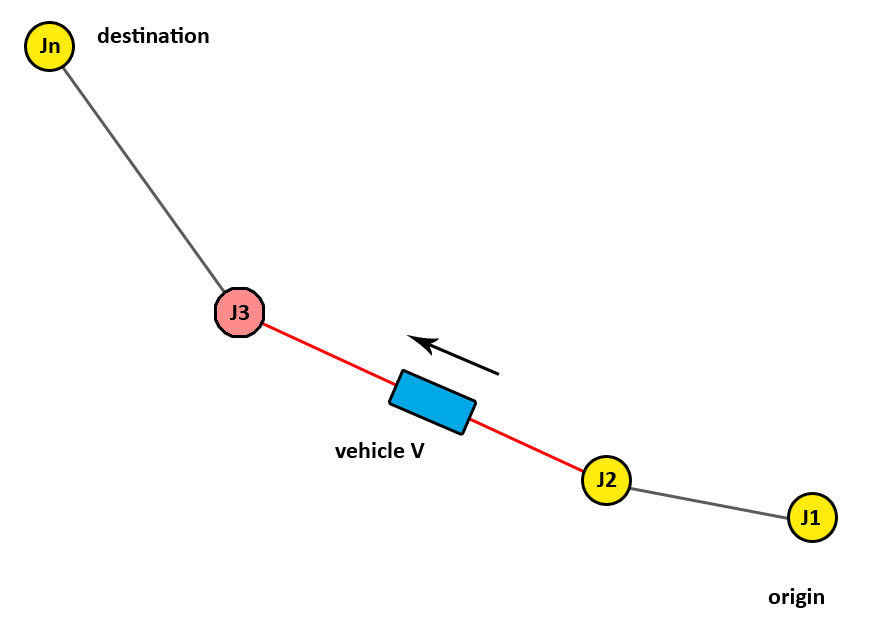
\includegraphics[scale=0.3]{moving_vehicles}
\caption{Vehicle V moving on its planned route.}
\end{center}
\end{figure}
\\

For example, consider Figure 7. The following are the main steps:
\begin{enumerate}
\item V is heading towards J3 so it needs to compute the distance to it. 
\item V computes its current displacement. Displacement is computed using a standard kinematics equation which takes into account velocity and acceleration.
\item There can now be two cases:
\begin{itemize}
\item If V cannot make it all the way to J3, V just moves towards it by the whole displacement in meters.
\item If V is close enough to J3, meaning that current displacement > distance to next junction, V first moves to J3, updates its route (i.e. a pointer to the next junction) and then performs the remaining displacement towards the new next junction.
\end{itemize}
\end{enumeration}



\subsubsection{Junction Classes}

Class Junction.java creates junction objects that are nodes on the road network. These objects contain references to road segments (including adjacent junctions and roads) and queues (containing vehicles) associated with it. It is used throughout the program to determine where vehicles are, and so is fundamental to vehicle behaviour.

Class TrafficLight.java extends Junction.java and schedules traffic light management. It has its own step method to iterate through lights, using class Light.java which encapsulates and toggles between the three light states.

In order to implement traffic management policies, some junctions need to embed special behaviour. Signal Green supports traffic light logic or give way signs, however the model can easily be expanded by extending the Junction class. We assume that junctions with more than two road segments need some traffic management logic, so they will be either instances of TrafficLight or GiveWaySign. (See Figures 8 and 9.)

Traffic lights have one instance of Light for each road adjacent to that junction, each light has a signal attribute which can be either RED or GREEN. Lights change their state every 25 ticks, at any time only one Light for that junction can be in GREEN state. Vehicles that are exiting a road segment check if the Junction is an instance of TrafficLight, in which case they inspect the signal to know if they must stop.
\\

\begin{figure}[H]
\begin{center}
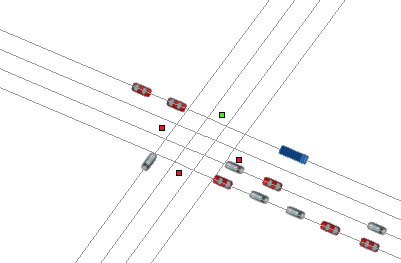
\includegraphics[scale=0.4]{traffic_light_junction}
\caption{Junction of type TrafficLight.}
\end{center}
\end{figure}

\\
In proximity of give way intersections, on the other hand, vehicles check for each road segment which vehicle is closest to that intersection, to know who has precedence.
\\
\begin{figure}[H]
\begin{center}
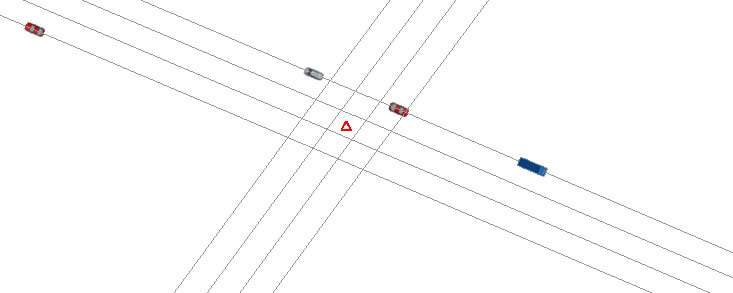
\includegraphics[scale=0.3]{give_way_junction}
\caption{Junction of type GiveWaySign.}
\end{center}
\end{figure}
\\

\subsection{External libraries and tools}

Most external libraries used are part of the Repast Simphony ABM toolkit.
The following list summarises the third party libraries used, some of which come with the installation of SG.
\begin{itemize}\itemsep0pt
\item Repast Simphony, free open source agent-based modelling platform.
\\
http://repast.sourceforge.net/

\item GeoTools, The Open Source Java GIS Toolkit, to read in GIS shapefiles.
\\
http://www.geotools.org/

\item OpenGIS Styled Layer Descriptor, free and publicly available, for rendering maps and vehicles.
\\
http://www.opengeospatial.org/standards/sld

\item JTS Topology Suite from Vividsolutions, an API of 2D spatial functions, open source, LGPL license.
\\
http://www.vividsolutions.com/jts/JTSHome.htm

\item GIS maps downloaded from the US Dept. of Transportation, freely available for download.
\\
http://www.fhwa.dot.gov/planning/processes/tools/nhpn/2011/

\item PriorityBlockingDeque, a doubly linked priority queue implementation by Aviad Ben Dov, based on java.util.concurrent.LinkedBlockingDeque.

\item IzPack java installer generator, for final project package. 
\\
http://izpack.org/

\end{itemize}


\subsection{Other Work}

The only class which is not our team\textquoteright s work is class PriorityBlockingDequeue.java. This class is copyrighted by Aviad Ben Dov, and it implements a rather complicated data structure holding vehicles in a queue at junctions. We used his work because the code was complex enough that it would take a great deal of time to write ourselves, and we thought it prudent to use his code with attribution instead of risking not completing the junction code satisfactorily in time or relying too heavily on his work.



\section{TESTING}



\subsection{Introduction}
This test plan has been created to check if our system conforms to all functional requirements and also to specify the testing techniques which will be used to validate the requirements of the system. Exhaustive testing of the system is naturally not realistically possible in the time given but we will use a diverse range of tests to find bugs and errors in the system including unit, functional, error and system testing. System is implemented using java therefore cross platform testing will be performed too. Automation testing will not be possible due to the nature of agent-based modelling simulations. Agents are non-deterministic and there is no set predictability of where objects will be at a given time. There is not a set result that can be expected for each vehicle, so automated testing for agents is not generally possible.

\subsection{Objectives and Tasks}
\subsubsection{Objectives}
The objective of testing our system is to provide adequate testing of functional requirements, validation and behaviour of system under simulated condition. Testing will be done by running the simulation, observing the agents' behaviour and comparing it with expected behaviour. Debug methods are written to eliminate bugs in the code which also form part of Unit testing as methods are smallest units of code in our system. All the exceptions are handled to avoid the crashes during simulation. 
Functional requirements are validated against the initial report.
Simulation is run atleast more than 3 times in order to test the expected behaviour of agents during simulation run to make sure that errors and bugs can be found and fixed.

\subsubsection{Tasks}
\begin{itemize}
\item Identifying functional requirements and writing the tests cases

\item Executing tests

\item Record the failed test cases and reporting them to team

\item Performing the re-test on failed test cases one bugs are fixed
\end{itemize}

\subsection{Scope}
In context to our system, which is implemented using agent-based model it will be tested at three different levels of functionality.
\begin{itemize}
\item Agents' behaviour\hfill \\
Verified by checking the changing environment variables around agents. This tests functional requirements of the system as well.\hfill \\

\item Runtime Parameters\hfill \\
Elements and data which load at runtime will be tested using valid and invalid inputs and checking for correct results. \hfill \\

\item Overall behaviour of system\hfill \\
Checks that all agents of the system produce expected results for a given scenario.\hfill \\

\end{itemize} 



\subsubsection{Levels of Functionalities}
\begin{itemize}%begin itemize for 3 levels

\item \textbf{Agents' behaviour: } \hspace \\ %Item 1
Can be checked by changing environment variables around agents. These behaviours of agents also forms the functional requirements of the system as well. We have two agents in our system. 

\begin{enumerate}%begin enumerate
\item\textbf {Vehicles}
step() method of Vehicle class is the entry point of control into simulation. All methods related to vehicle behaviour are invoked inside this method.\hfill \\



\begin{itemize} %Itemize for test cases
\item \textbf{Test Case1:} \hspace{6 mm} Vehicle Impasse\hfill \\
\underline{Expected Output: }\hspace{6 mm}This "if condition" in step() method should not be true i.e. no Vehicle should be stuck in impasse.\hfill \\
\underline{Actual Output:} \hspace{6 mm}Console output does not print the statement "Vehicle is stuck in impasse. Cannot move...". "if condition" remains false.\hfill \\
\underline{Result:} Passed\hfill \\



\item \textbf{Test Case 2:} \hspace{6 mm}moveTowards()\hfill \\
\underline{Input:} \hspace{6 mm}Coordinate and displacement\hfill \\
\underline{Expected Output:} \hspace{6 mm}Every vehicle on the network should move to a new coordinate and exception should not be thrown printing on console "Could not move vehicle for some reason.". \hfill \\
\underline{Actual Output:} \hspace{6 mm}Vehicle moved. No exception thrown.\hfill \\
\underline{Result:} \hspace{6 mm}Passed\hfill \\
\item \textbf{Test Case 3:} \hspace{6 mm}Accelerate() Every vehicle must accelerate in order to move.\hfill \\
\underline{input:} \hspace{6 mm}Takes ACCELERATION and time t to calculate velocity.\hfill \\
\underline{Expected Output:} \hspace{6 mm}Vehicles should be moving not more than maximum velocity.\hfill \\
\underline{Actual Output:} \hspace{6 mm}No vehicle colliding and no vehicle static if car ahead is not stopping.\hfill \\
\underline{Result:}Passed\hfill \\

\item \textbf{Test Case 4:} \hspace{6 mm}slowDown()Every vehicle must slow down in order to stop.\hfill \\
\underline{Input:} \hspace{6 mm}Takes ACCELERATION and t*2 to calculate velocity.\hfill \\
\underline{Expected Output:} \hspace{6 mm}If velocity is less than zero then vehicles must stop.\hfill \\
\underline{Actual Output:} \hspace{6 mm}Vehicles stopped when velocity is less than zero.\hfill \\
\underline{Result:} \hspace{6 mm}Passed\hfill \\
\end{itemize}%end itemize
\item\textbf{Traffic Lights}
\begin{itemize} %itemize for test cases
\item \textbf{Test Case 5:} Traffic Light Green \hfill \\
\underline {Expected Output:}Cars should keep moving if traffic light is green.\hfill \\
\underline{ Actual Output:}Cars did not stop.\hfil \\
\underline{ Result:}Passed.

\item \textbf{Test Case 6:} Traffic Light Red\hfill \\
\underline{Expected Output:} Cars should stop if traffic light is red.\hfill \\
\underline{ Actual Output: }Cars stops when traffic light is red.\hfill \\
\underline{Result:} Passed
\item \textbf{Test Case 7:} Traffic Lights On More Than 2 Roads Junction\hfill \\
Traffic lights should only be displayed on junctions that contain more than two roads.\hfill \\
\underline{Expected Output:} Only junctions with more than two roads display traffic lights.\hfill \\
\underline{Actual Output:} Traffic lights are displayed only on more than two road junctions.\hfill \\
\underline{Result:} Passed\hfill \\
\end{enumerate}

\begin{figure}[h!]
\centering
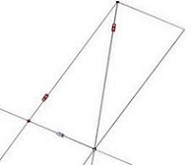
\includegraphics{junction}\hfill \\
Network with traffic lights.
\end{figure}
\end{itemize}


\item \textbf{Runtime Parameters:} 

Elements and data which loads at run time will form part of runtime testing. It will be tested, giving all valid and invalid inputs and check results. Following elements will be tested at run time:


\begin{itemize}%Test cases itemize
\item \textbf{Test Case 8:} SignalGreenBuilder Implements ContextBuilder\hfill \\
This class contains methods to build the context and initialise all variables required during the simulation execution.\hfil \\
\underline{Input:} Run signalGreen Model, to load user GUI which contains GIS map, Vehicle agents and TrafflicLight Agents.\hfill \\
\underline{Expected Output:} Map should be loaded and displayed along with three different types of vehicles and traffic lights on all junctions that have more than two edges.\hfill \\
\underline{Actual Output:} Map loaded with 100 vehicles which is default value and traffic lights on junctions with more than two edges only.\hfill \\
\underline{Result:} Passed\hfill \\

\item\textbf{Test Case 9:} Number of vehicles\hfill \\
\underline{Input:} Enter a number in "Number of vehicles" field on parameters tab.\hfill \\4, 0 , -1 and a character given as input.\hfill \\
\underline{Expected Output:} Only entered number of vehicles should appear on road network. No vehicles should appear for negative numbers and characters. \hfill \\
\underline{Actual Output:} Vehicles are equal to number entered. No vehicles for negative and character input.\hfil \\
\underline{Result:} Passed\hfill \\
\begin{table}[H]
\begin{center}
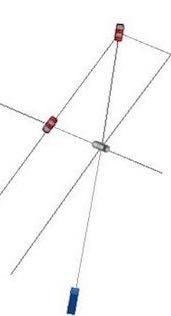
\includegraphics[scale=0.8]{4Cars}\hfill \\
4 Vehicles on the road
\end{center}
\end{table}
\item \textbf{Test Case 10:} No Traffic Lights\hfill \\
"Traffic Lights" on parameters tab, if unchecked traffic lights should not appear on display and cars should not consider traffic lights.\hfill \\
\underline{Expected Output:} Cars should travel on road without stopping at traffic lights as there are none.\hfill \\
\underline{Actual Output:} No traffic lights are displayed and cars carry on moving on roads.
\underline{Result:}Passed.\hfill \\ 
\item \textbf{Test Case 11:}Multiple Maps\hfill \\
\underline{Input:}In parameters tab, user should be able to select different maps. Manhattan and New York maps given as input. \hfill \\
\underline{Expected Output:} Maps should be loaded at run time and simulation should run.\hfill \\
\underline{Actual Output:}Two different maps loaded and simulation executed successfully.\hfill \\
\underline{Result:}Passed\hfill \\
\begin{table}[H]
\begin{center}
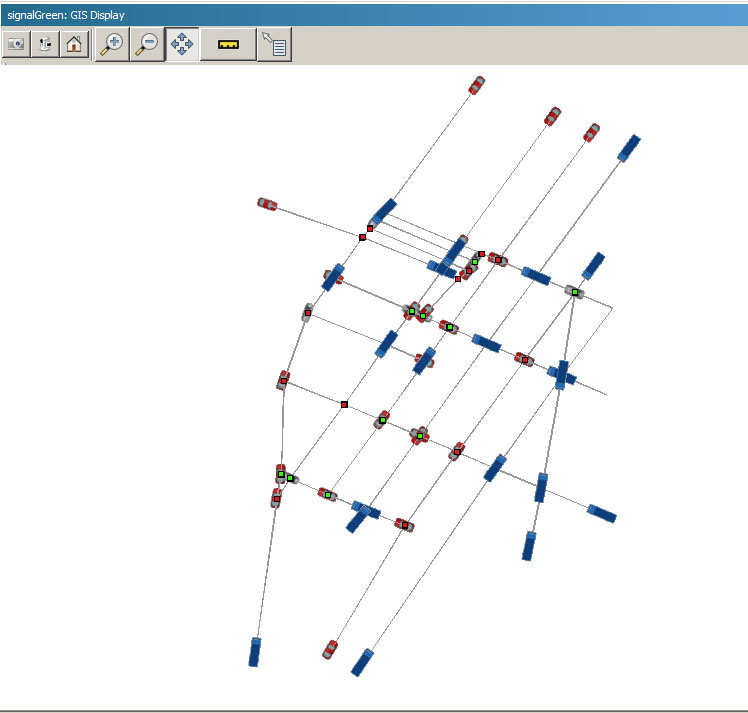
\includegraphics[scale=0.4]{manhattan_section}\hfil \\
GIS Map for Manhattan
\end{center}
\end{table}
\begin{table}[H]
\begin{center}
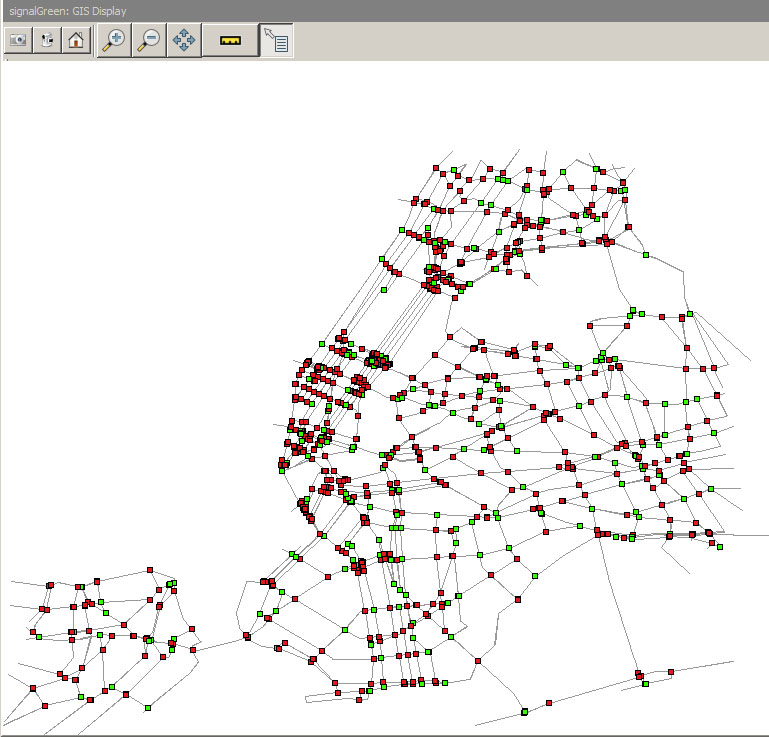
\includegraphics[scale=0.4]{nyc_full}\hfill \\
GIS Map for New York
\end{center}
\end{table}
\end{itemize}%Test cases itemize


\item \textbf{Overall behaviour of system: }%Item 3
Checks that all agents of the system produce expected results in a given scenario. This will include testing of agents interaction with other components of environment (roads, traffic lights) when programme will be executed at run time.\hfill \\
\begin{itemize}%Test case itemize
\item \textbf{Test Case 12:} Every junction holds a queue of vehicles running on a particular outward road.\hfill \\
\underline{Expected Output:} of next.printVehiclesQueue(origin):[signalGreen.Vehicle@54008645, signalGreen.Vehicle@1a43b86b] Peek vehicle: signalGreen.Vehicle@54008645\hfill \\
\underline{Actual Output: }Using probe tool, selecting the area which we want to inspect:\hfill \\
There are indeed two vehicles running on W 34th St, and their object ID match.\hfill \\
\underline{Result: }Passed\hfill \\
\begin{figure}[h]
\begin{center}
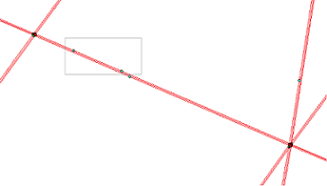
\includegraphics[scale=0.7]{RoadNetwork}\hfill \\
Two vehicles using select tool.
\end{center}
\end{figure}
\begin{table}[H]
\begin{center}
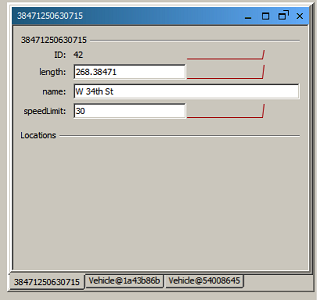
\includegraphics{Sim}\hfill \\
Vehicles' IDs
\end{center}
\end{table}
\item \textbf{Test Case 13:} Multilanes and Bi-directional Roads\hfill \\
\underline{Expected Output:}Each road should have two lanes in each direction and vehicles should be able to change lanes.\hfill \\
\underline{Actual Output:}Multilane roads loaded and fast vehicles took over slow ones by changing lanes.\hfill \\
\underline{Result:}Passed
\end{itemize}%Test case itemize


\end{itemize}%End itemize for 3 functionalities.
\subsection{Performance Requirements}
System has been tested on two operating systems, Windows7 and MAC OX(Yosemite).All three machines have 8GB RAM and i3 and i5 and i7 processors. System responded in acceptable time but simulation takes longer time to be processed by CPU when number of vehicles are increased.\hfil\\
In general, execution speed of simulation will depend on processor and RAM of the system on which it will be running.
\subsection{Conclusion}
This test plan covers all major requirements of traffic simulation we have developed which verifies the functional requirements established at the beginning of the project. Test cases were developed to test the expected behaviour of the system using different parameters at run time.




\section{TRAFFIC POLICY COMPARISON}


\subsection{Data Extrapolation}


Data extrapolation was implemented into the simulation allowing for comparisons of difference and efficiency between various maps that the simulation emulates. The implementation begins by recording data from data sources. These are predefined as aggregate or non-aggregate. They have been created with linked hash maps that use Repast’s integrated ability to pass agents and objects towards the correct data source. For example, the simulation model records an aggregate data source for average speed by calling the getVelocity() method of all vehicle agents in the simulation at each time step. The aggregate operation attains the mean value from the results of getVelocity(). 

To assist in creating reporting, Repast has an XML data set descriptors. Descriptor repast.simphony.data2.engine.DataSetDescriptor defines the datasets being created, and it has an integrated ability to create charts from these defined data sources using descriptor repast.simphony.chart2.engine.TimeSeriesChartDescriptor.

To visualize the extrapolated data being collected from the data sources, the data is plotted against tick count on a time series chart. For example, to view the average speed of vehicles the Simphony descriptor was used to define attributes on a time series chart, where the x-axis has the tick count and y-axis has the mean speed. (See Figure 1XXXXX.) The descriptor is defined in XML and is repast.simphony.chart2.engine.TimeSeriesChartDescriptor.

 

Figure 1xxxxx. Time series chart for average speed calculated at tick count.

The simulation stores data collected from the data sources and writes the data into a sink text file. This makes use of Repast’s ability to write data to both file and console. Each data source is assigned a data set ID which helps separate out the data and write each ID in a set column. 

The follow shows resultant data stored for average speed. As seen in the output, the sink file structures the data collected from each data source in a tabular format. 

\begin{center}
\begin{tabular}{ l | r  }
\hline
Average Speed & Tick \\
1.1900000000000002 & 1.0 \\
2.380000000000003  &  2.0 \\
3.5699999999999985 & 3.0 \\
\hline
\end{tabular}
\end{center}

Figure 2xxx. Signal Green simulation output.




\subsection{Policy Comparisons}

The simulation was used with several parameters and maps to allow for road network and policy comparisons. Three maps was being used presently, large New York, small New York and New Jersey. What is being examined presently is the change in behaviour when the following parameters are adjusted; number of vehicles, traffic lights and give way signs. The data being extrapolated to analyse change is the speed of the vehicles.


\subsubsection{New York map}


Small New York map (nyc\_small.shp) covers an area of approximately 20 sq km. Our simulation models only main roads. 

10,000 vehicles to account for peak hours and 1,000 to simulate late night.


Figure 3xx. Legend displaying palette used to visualise speed of individual vehicle agents in the simulation.

Traffic lights policy was simulated on this map with parameters set as 10,000 vehicles and 1000 ticks. The data shows a gradual increment of average speed to a maximum of 41. It also shows very heavy concentration is being built up at junctions.
Figure xx.
Figure xx.

1,000 vehicles and 1000 ticks. With these parameters the data shows a sharp increase in average speed to a maximum of 95. The data shows dense concentration across popular routes and junctions.
Figure xx.
Figure xx.

Give way policy was simulated on this map with parameters set as 1,000 vehicles and 1000 ticks. This led to one of the fastest average speed recorded with it being a maximum of 110. The data shows similar density to the traffic lights policy with the same number of vehicles.
Figure xx.
Figure xx.

10,000 vehicles and 1000 ticks was not carried out as the simulation would not accurately cope with such a high density of vehicles. In actuality vehicles could potentially suffer accidents that have yet to be modelled. 

The following is a summary in tabular form for policies tested on this map:


\begin{center}
\begin{tabular}{ l | c | c | c }
\hline
Policy & No. of Vehicles & Ticks & Average Speed \\
Traffic Light & 10,000 & 1,000 & 40 \\
Give Way & 10,000 & 1,000 & - \\
Traffic Light & 1,000 & 1,000 & 88 \\
Give Way & 1,000 & 1,000 & 105.7 \\
\hline
\end{tabular}
\end{center}

SignalGreen shows us that average speed with give way policies is higher because cars need to stop less frequently than when with traffic lights. Moreover, the difference in distribution between give way and traffic light policies when using a 1,000 vehicles has no significant difference.

Our data shows that give way policies would be more desirable for traffic flow. While officials might think it would be perhaps too risky in more densely populated areas such Manhattan, perhaps this is an area that city planner should consider in future development.

\subsubsection{New Jersey map}

New Jersey map (new\_jersey.shp)  covers a much more complex infrastructure. Below it is set at 2,000 vehicles with 1000 ticks to analyse the give way and traffic light policies.

Traffic lights policy was simulated on the model where the data shows a steep climb to the maximum average speed of 110 and then remaining around 105. Traffic lights do become congested with queues

Figure xx.
Figure xx.

The give way policy was then run using the same parameters and the result was a constant average speed of 110. Vehicles were scattered evenly with only a small number of queues. present.
Figure xx.
Figure xx.

The following is a summary in tabular form for policies tested on this map:
\begin{center}
\begin{tabular}{ l | c | c | c }
\hline
Policy & No. of Vehicles & Ticks & Average Speed \\
Traffic Light   & 2,000     &          1,000 &     105  \\
Give Way     &   2,000  &             1,000    &  100 \\
\hline
\end{tabular}
\end{center}

\subsection{Policy Comparison: Conclusion}

Our simulation implemented different traffic policies and measured the difference between them, both with numerical data and graphically. Our simulation indicates that give way policies may be a useful policy to consider implementing for smoother traffic flow and overall better travel time for drivers.

In future, there are alternative ways that can be used to analyse traffic policies. For instance, computing routes or segments that are most popularly travelled by vehicles. Also, busiest intersections that lie between those very routes. It is also important to simulation using a combination of these policies such as traffic lights and give way signs to look into the further potential of these policies.




\section{TEAM WORK}

Our approach to the project was to set down ideas, goals, and tools in the first two weeks, then jump into the coding and get as far along as we could until the initial report came due. This worked well in many ways. Important decisions about implementation were decided very quickly so coding was able to start in January. The milestones were itemized early in the project, with Milestone 1 set early and items assigned to Milestones 2 and 3 differentiated closer to the deadline of the Initial Report.


\subsection{Roles and Task Division}

\begin{description}
\item [Waqar Aziz] \hspace{16 mm} Developer Two, Head Policy Comparison and Reporting \\
	Develop reporting functionality; primary traffic policy testing and reporting; design Junction class
\item[James Kerr] \hspace{16 mm}  Documentation Specialist Two, LaTeX Specialist \\
	Writing technical documentation for report
\item[Adeela Saalim] \hspace{11 mm} Testing Specialist \\
	Develop test cases, run test cases, document testing
\item[Andrea Senf] \hspace{15 mm} Team Coordinator, Tech Doc Specialist \\
	Coordinate team activity, Scrum Master, Lead documentation and reporting
\item[Yoann Strigini] \hspace{11 mm}  Design Architect, Developer One \\
	Design SignalGreen model, integration with GIS, develop Vehicle class, presentation layer
\end{description}

\subsection{Tools}

\begin{itemize}\itemsep0pt
\item GitHub. GitHub was used for creating the code, providing version control and easy sharing of code. Initial and final reports were also kept there. Andrea held the main code repository, and the team branched off that code.
\item Communication. For communication outside coding, the most used tool by far was WhatsApp; this was practical for team chat, answering basic questions, and coordinating meetings. Longer reports for the group were written on asana or sent by email. Asana was used consistently by team members and was helpful for the documentation of the final report and for automatically generated Gantt charts through Instagantt.
\item Meetings. When one or more group members believed a whole group meeting was needed to further the project, this was communicated on WhatsApp and a time and place of meeting was arranged using input from all members. These meetings were in person. Other times two or three members met together using Skype or in person as needed to work on parts of the project pertaining only to them.
\end{itemize}



\subsection{Development and Reporting}

The team set out to utilize an Agile method of development with SCRUM reports once a week, either in person (if we had a meeting) or written if we did not gather. Group SCRUM did not pan out exactly as anticipated, as early meetings had absences which made SCRUM impractical as we waited for other members arrived (which they occasionally did not). We then decided to transition completely to written reports. 

Approximately every week the group coordinator would remind the team to post WhatsApp/asana updates so everyone was aware of what the others were doing and to help the team to continually progress. Team members were to request help as needed and there was always a visible \textquoteright next task \textquoteright\ waiting when one\textquoteright s current task had been completed, so while SCRUM was not overtly performed the goals behind the method did remain.


\subsection{Team Challenges}

Our team faced several challenges in working together and with our chosen tools. [Note: all members are here referred to as \textquoteright he\textquoteright .] 

\begin{itemize}\itemsep0pt
\item Our team struggled to coordinate regarding GitHub the first part of the project, as several members focused on coding on their own machines rather than branching from GitHub in the weeks prior to the initial report date. Initial code was uploaded to GitHub the day before the initial report was due. The members leading in coding later created a full GitHub project for everyone to access. 
\item A member missed two meetings where decisions were made, so his preferences were not implemented. As he had strong feelings about these decisions it was difficult for the person to accept and caused some friction.
\item A member found he did not have the ability to run Simphony and so did not have a way to code his part of the project; the group was notified of this after the initial report presentation. He found a way to partially resolve this so he could code from the last week of February, although still without full Eclipse functionality. 
\item A member had difficulty prioritizing his code at the end, putting off resolving a key issue for several days. This resulted in our final Milestone deadline being pushed back almost a week and added stress to other team members.
\item After difficulty getting team members to follow through with attending agreed meetings, we voted to modify our practice so that absence to agreed full group meetings would result in a point for that person being deducted.
\end{itemize}
\\


\section{EVALUATION}


\subsection{Group Project}

University group projects can be tricky to make work well; professional teams generally have the benefits of prior working relationships and clearly understood authority and accountability structures. SignalGreen team members were generally unfamiliar with each other before forming the group; four of our team formed based on where we were sitting in the introductory lecture, and the fifth was a person who we heard was looking for a group. 

Distributing points is generally difficult to manage well, as giving too much power to democratic vote can be seen as unfair and hurtful by some members, and not allowing enough flexibility can result in members not feeling impressed to participate or work in a timely fashion. 

In general, as masters students we are committed to doing good work, as our work for the project is part of our training for our careers. On this basis our team decided to share points evenly, and points lost due to agreed criteria would be distributed by vote. Some members did more work than our points can reflect, and we trust their hard work will pay off in personal dividends in the future.

Ultimately, the goal of the team was for everyone to get through the module with a pass (preferably much better). To this end, we are not group critiquing each other, nor are we calculating what we ourselves did for comparison to others. As we believe our team has been successful in the project we feel it would be better to end with a feeling of satisfaction for having completed a quality project.


\subsection{Milestone Results}

All objectives set for Milestone 1 were completed in its entirety by the deadline set by the team. At that time we extended the deadlines of the Milestones to have all coding finished by 16 March, and then turn to cleaning the code and final commenting while testing was finishing and traffic policies were compared during the week of 16 March.
\\
We completed tasks very close to the schedule we set out at the beginning. In the interest of better code, we extended the Milestone 2 deadline to March 16; this allowed some desired behaviours to be completed. All coding was originally scheduled to stop 16 March to leave time for continued testing, commenting and code cleaning, and documentation. 

A team member had issues with his code that put the team a week behind at the end. This was disappointing, but team members pulled together to complete the rest of the tasks on schedule and bring out our traffic simulation by the deadline.
\\

\subsection{Final Characteristics from Milestone Requirements}
\begin{itemize}
\item vehicles run on a map
\item multiple maps in GIS standard
\item variable number of vehicles
\item vehicles make decisions to reach a goal
\item vehicles exhibit passing behaviours 
\item implement basic vehicle types: car, lorry
\item cars have different behaviours: aggressive, patient
\item vehicles appear visually different by type
\item traffic flows bi-directionally
\item junctions, signals, give way 
\item multiple lanes on some/all roads
\item speed limits on roads
\end{itemize}



\subsection{Functional Requirements Coverage}

Out of these requirements we did not compete 1) FR4.4 junction roundabout functionality, 2) FR4.6 orange signal functionality, and 3) FR2.4 Vehicles follow speed limit of roads. The give way and signal code took longer to implement than we originally thought, so we did not continue on to roundabouts; this will be something interesting to add at a future time. Orange light functionality was partially completed, but it was dropped by the team because it was an optional functionality and the simulation did not require it. Speed limits functionality was partially implemented, as the GIS maps we used did not have such attribute to use, so currently it arbitrarily defaults to the maxVelocity of vehicles.

\subsection{Project Acceptance Criteria}

The project is deemed as success in that all coverage criteria have been met.
The following table lists all criteria used to assess the project, and their pass/fail criteria

\begin{table}[h]
\begin{tabular}{lll}
Coverage Criteria & Total Covered & Pass/Fail \\
High Priority Requirements implemented \textgreater= 100\% & 100\% & Pass \\
Low Priority Eequirements implemented \textgreater= 70\% & 100\% & Pass \\
Functional Requirements tested success \textgreater= 80\% & 90\% & Pass \\
SCRUM meeting attendance \textgreater= 70\% & 70\% & Pass \\
At least SG v2.0 has been released & Released SG v3.1 & Pass \\
Total GitHub commits \textgreater 200 & More than 250 & Pass \\
Comments and Javadoc covers more than 90\% code & 100\% & Pass \\
SG submitted on time or within extra submission time & On time & Pass
\end{tabular}
\end{table}


\begin{figure}
\begin{center}
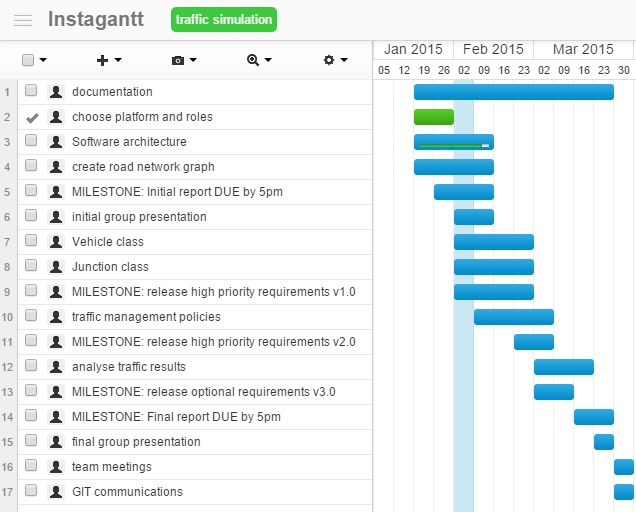
\includegraphics[scale=0.65]{gantt8Feb}
\caption{Gantt Chart from 8 Feb}
\end{center}
\end{figure}

\begin{figure}
\begin{center}
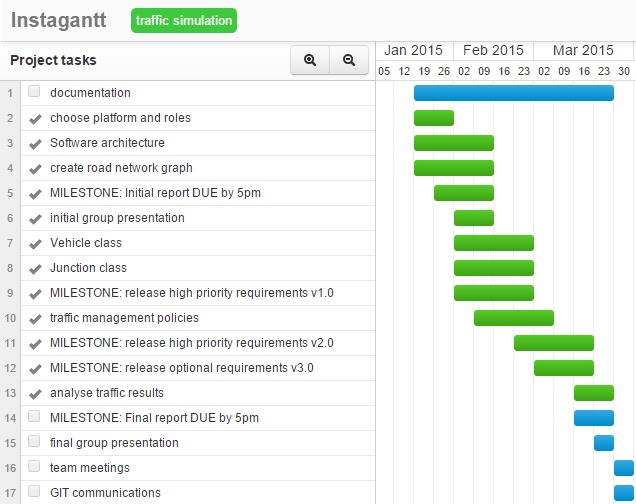
\includegraphics[scale=0.6]{gantt26Mar}
\caption{Gantt Chart from 26 March}
\end{center}
\end{figure}
\\


\subsection{Repast Simphony}

Overall we think our use of Repast Simphony was successful for our project. It provided a foundation API and Eclipse configuration that was not directly involved with agents or behaviours. It allowed us to create attractive visuals in the simulation and analysis graphing. We spent little time debugging, and were able to focus on simulating traffic. Simphony provided many extras (XML persistent storage, installers, etc) that we did not use due to lack of need or lack of implementation time.

An unforeseen disadvantage of Simphony arose in that it cannot be installed or used on KCL lab computers. One member of our group did not have access to Simphony at home or on campus (the group did not know this until after the initial presentation), and he was not able to find a way to use Simphony until almost March, and then not effectively. This greatly reduced his ability to be useful to the team in coding and held up work on a major segment of the code.

Originally we planned to use a belief-desire-intention (BDI) model to code the agents\textquoteright\ behaviour, but as the member intending to code this was unable to use Simphony, behaviours were instead coded into the agents themselves.
\\


\subsection{Further Work}

\textquotedblleft Validation data is usually macroscopic statistics such as flow rate, speeds and queue time, which can easily be compared with data from real traffic experiments. \textquotedblright \cite{4d} 

\begin{itemize}\itemsep0pt
\item If we had more time we would have liked to download a road map from a town in England where we know road data/statistics and compare our model to the actual traffic flow for the same road. This would be a big step in validating our logic and making the code useful to others wishing to model traffic.

\item Creating roundabouts was the next goal for our code, and this would make the code work for modelling most UK towns and cities. (Roundabouts are not generally used in the USA.)

\item Further development can be done in displaying road closures for modelling construction or traffic accidents. This would make the model more realistic and useful in determining maintenance disruption.

\item Implement source/sinks for allowing traffic to come on/off the map in a more natural location than at junctions; perhaps from the edges of the map would be more optimal visually. This would allow traffic congestion to increase as more cars are fed into the simulation than are going out (and vice versa), and would allow modelling of road conditions created by end of workday, post-sport competition, etc. 

\item We did not make progress on the BDI as planned, so this was left out of the code. The code could be restructured to more neatly implement this if desired.

\item Adding other vehicle types such as motorbikes or road features such as pedestrian crossings or high occupancy vehicle (HOV) lanes to model their effect on congestion and traffic flow.
\end{itemize}


\section{PEER ASSESSMENT}


Waqar: 19.5

James: 19.5

Adeela: 20

Andrea: 20

Yoann: 21


\newpage




\bibliographystyle{plain}
\bibliography{bibliography}


\newpage

\begin{appendices}


\appendix{Appendix A: GitLog}
%\chapter{Appendix A: Gitlog}

\begin{center}
\begin{longtabu} to \textwidth {|
X[4,l]|
X[3,c]|
X[8,l]|}
\hline
\textbf{Author} & \textbf{Date} & \textbf{Message} \ \hline
asenf & 2015-01-22 & first commit \\ \hline
asenf & 2015-01-22 & team members \\ \hline
asenf & 2015-01-22 & repo.txt \\ \hline
asenf & 2015-01-22 & Initial commit \\ \hline
asenf & 2015-01-22 & Merge origin/master \\ \hline
asenf & 2015-01-22 & License Header Update \\ \hline
Andrea Senf & 2015-01-22 & Initial Commit \\ \hline
asenf & 2015-01-28 & Initial Commit Eclipse Project \\ \hline
JamesWKerr & 2015-01-30 & testing push again \\ \hline
JamesWKerr & 2015-01-30 & sanity checking I can pull, modify code, and push \\ \hline
asaalim & 2015-01-30 & This is a test fiel \\ \hline
JamesWKerr & 2015-01-30 & Work! \\ \hline
JamesWKerr & 2015-01-30 & working on lab machine finally \\ \hline
asaalim & 2015-01-30 & Finally a textfile.txt \\ \hline
JamesWKerr & 2015-01-30 & trying nice merge \\ \hline
asaalim & 2015-01-30 & Changed Signal\_Green.java file \\ \hline
JamesWKerr & 2015-01-30 & Merge branch `master' of https://github.com/asenf/team\_SignalGreen \\ \hline
JamesWKerr & 2015-01-30 & nastyMerge \\ \hline
JamesWKerr & 2015-01-30 & tryingToBreakGitMerge \\ \hline
asaalim & 2015-01-30 & checking merge \\ \hline
asaalim & 2015-01-30 & conflict resolved \\ \hline
asenf & 2015-02-01 & Merge remote-tracking branch `origin/master' \\ \hline
asenf & 2015-02-01 & upload reports, delete txt files \\ \hline
asenf & 2015-02-01 & add report \\ \hline
asenf & 2015-02-01 & license header update \\ \hline
asenf & 2015-02-01 & delete EclipseProject \\ \hline
asenf & 2015-02-03 & update initial report \\ \hline
asenf & 2015-02-03 & update initial report \\ \hline
JamesWKerr & 2015-02-05 & trying out fancy new phone git app if some people are gonna use abstracted GUIs or plugins, this will beat them I think \\ \hline
yo-stri & 2015-02-07 & Update LaTeXv2.tex \\ \hline
JamesWKerr & 2015-02-08 & cleaned up repo heirarchy \\ \hline
JamesWKerr & 2015-02-08 & Merge branch `master' of https://github.com/asenf/team\_SignalGreen \\ \hline
asenf & 2015-02-08 & Most recent initial report. \\ \hline
asenf & 2015-02-08 & coordinator.txt for inital report \\ \hline
asenf & 2015-02-08 & most recent initial report, version 5 \\ \hline
asenf & 2015-02-08 & coordinator.txt for initial report \\ \hline
asenf & 2015-02-08 & coordinator.txt for initial report \\ \hline
asenf & 2015-02-08 & coordinator.txt for initial report \\ \hline
asenf & 2015-02-08 & version 5 \\ \hline
JamesWKerr & 2015-02-09 & packages \\ \hline
JamesWKerr & 2015-02-09 & Merge branch `master' of https://github.com/asenf/team\_SignalGreen \\ \hline
JamesWKerr & 2015-02-09 & morePackageLayout \\ \hline
JamesWKerr & 2015-02-09 & morePackageOrgqnisqtion \\ \hline
JamesWKerr & 2015-02-09 & adding to gitignore \\ \hline
asenf & 2015-02-09 & initial presentation - Andrea \\ \hline
asenf & 2015-02-09 & initial presentation - Andrea \\ \hline
asenf & 2015-02-09 & commit \\ \hline
asenf & 2015-02-09 & commit \\ \hline
asenf & 2015-02-09 & commit \\ \hline
asenf & 2015-02-09 & commit Adeela presentation \\ \hline
yo-stri & 2015-02-09 & Create Vehicle.java \\ \hline
yo-stri & 2015-02-09 & Create Utils.java \\ \hline
yo-stri & 2015-02-09 & Create SignalGreenBuilder \\ \hline
yo-stri & 2015-02-09 & Create Constants.java \\ \hline
yo-stri & 2015-02-09 & Create Junction.java \\ \hline
yo-stri & 2015-02-09 & Create TrafficLight.java \\ \hline
yo-stri & 2015-02-09 & Rename signal\_green/src/signalGreen/Constants.java to signal\_green/src/signalGreen/src/Constants.java \\ \hline
yo-stri & 2015-02-09 & Rename signal\_green/src/signalGreen/Junction.java to signal\_green/src/signalGreen/src/Junction.java \\ \hline
yo-stri & 2015-02-09 & Rename signal\_green/src/signalGreen/SignalGreenBuilder to signal\_green/src/signalGreen/src/SignalGreenBuilder \\ \hline
yo-stri & 2015-02-09 & Rename signal\_green/src/signalGreen/TrafficLight.java to signal\_green/src/signalGreen/src/TrafficLight.java \\ \hline
yo-stri & 2015-02-09 & Rename signal\_green/src/signalGreen/Utils.java to signal\_green/src/signalGreen/src/Utils.java \\ \hline
yo-stri & 2015-02-09 & Update Utils.java \\ \hline
yo-stri & 2015-02-09 & Update and rename signal\_green/src/signalGreen/Vehicle.java to signal\_green/src/signalGreen/src/Vehicle.java \\ \hline
yo-stri & 2015-02-09 & Create context.xml \\ \hline
yo-stri & 2015-02-09 & Merge pull request \#3 from asenf/yoann \\ \hline
yo-stri & 2015-02-09 & Rename signal\_green/src/signalGreen/src/Constants.java to signal\_green/src/signalGreen/Constants.java \\ \hline
yo-stri & 2015-02-09 & Rename signal\_green/src/signalGreen/src/Junction.java to signal\_green/src/signalGreen/Junction.java \\ \hline
yo-stri & 2015-02-09 & Rename signal\_green/src/signalGreen/src/SignalGreenBuilder to signal\_green/src/signalGreen/SignalGreenBuilder \\ \hline
yo-stri & 2015-02-09 & Rename SignalGreenBuilder to SignalGreenBuilder.java \\ \hline
yo-stri & 2015-02-09 & Rename signal\_green/src/signalGreen/src/TrafficLight.java to signal\_green/src/signalGreen/TrafficLight.java \\ \hline
yo-stri & 2015-02-09 & Rename signal\_green/src/signalGreen/src/Utils.java to signal\_green/src/signalGreen/Utils.java \\ \hline
yo-stri & 2015-02-09 & Rename signal\_green/src/signalGreen/src/Vehicle.java to signal\_green/src/signalGreen/Vehicle.java \\ \hline
yo-stri & 2015-02-09 & Rename signal\_green/src/signalGreen/SignalGreen.rs/context.xml to signal\_green/SignalGreen.rs/context.xml \\ \hline
yo-stri & 2015-02-09 & Rename signal\_green/SignalGreen.rs/context.xml to signalGreen/SignalGreen.rs/context.xml \\ \hline
yo-stri & 2015-02-09 & Rename signal\_green/src/signalGreen/Constants.java to signalGreen/src/signalGreen/Constants.java \\ \hline
yo-stri & 2015-02-09 & Rename signal\_green/src/signalGreen/Junction.java to signalGreen/src/signalGreen/Junction.java \\ \hline
yo-stri & 2015-02-09 & Rename signal\_green/src/signalGreen/SignalGreenBuilder.java to signalGreen/src/signalGreen/SignalGreenBuilder.java \\ \hline
yo-stri & 2015-02-09 & Rename signal\_green/src/signalGreen/TrafficLight.java to signalGreen/src/signalGreen/TrafficLight.java \\ \hline
yo-stri & 2015-02-09 & Rename signal\_green/src/signalGreen/Utils.java to signalGreen/src/signalGreen/Utils.java \\ \hline
yo-stri & 2015-02-09 & Rename signal\_green/src/signalGreen/Vehicle.java to signalGreen/src/signalGreen/Vehicle.java \\ \hline
yo-stri & 2015-02-09 & Merge pull request \#4 from asenf/yoann \\ \hline
asenf & 2015-02-09 & delete duplicates \\ \hline
asenf & 2015-02-09 & delete duplicates \\ \hline
asenf & 2015-02-10 & initial report final \\ \hline
asenf & 2015-02-10 & proofread \\ \hline
asenf & 2015-02-11 & Update TrafficLight.java \\ \hline
asenf & 2015-02-11 & pdf presentation \\ \hline
yo-stri & 2015-02-11 & Update Constants.java \\ \hline
yo-stri & 2015-02-11 & Merge pull request \#5 from asenf/test \\ \hline
James William Kerr & 2015-02-12 & my role in this \\ \hline
yo-stri & 2015-02-13 & creating the whole runnable project \\ \hline
yo-stri & 2015-02-14 & multiple vehicles running on simulation \\ \hline
yo-stri & 2015-02-14 & vehicles can now accelerate according to their max velocity \\ \hline
yo-stri & 2015-02-14 & vehicles can accelerate or slow down according to distance to junctions \\ \hline
yo-stri & 2015-02-14 & some minor updates to the Vehicle acceleration functionality \\ \hline
asenf & 2015-02-17 & test \\ \hline
waqaraaziz & 2015-02-18 & Removed comment \\ \hline
waqaraaziz & 2015-02-18 & Added multilane implementation with comments \\ \hline
waqaraaziz & 2015-02-18 & Updated with new junction approach and comments \\ \hline
waqaraaziz & 2015-02-18 & Updated lights with new multi-lane implementation \\ \hline
waqaraaziz & 2015-02-18 & Merge pull request \#8 from asenf/multiple-lanes \\ \hline
yo-stri & 2015-02-18 & added more edges and made some mods to the vehicle class \\ \hline
waqaraaziz & 2015-02-19 & Added weight parameter to addLane method \\ \hline
waqaraaziz & 2015-02-19 & Added weight parameter to addLane method \\ \hline
waqaraaziz & 2015-02-19 & Added addJunction, buildComplexJunctionsAndLanes() \\ \hline
JamesWKerr & 2015-02-19 & rough sketch, finally got peristant windows vm on external hdd working, so many more improvements to come \\ \hline
JamesWKerr & 2015-02-19 & organizing of formal algorithm into java. Hoping to have basic behaviour done tomo \\ \hline
JamesWKerr & 2015-02-19 & Merge branch `master' of https://github.com/asenf/team\_SignalGreen \\ \hline
waqaraaziz & 2015-02-19 & Light object for Traffic Lights \\ \hline
waqaraaziz & 2015-02-19 & Change enum to prevent conflict \\ \hline
waqaraaziz & 2015-02-19 & Implemented Light object and algorithms \\ \hline
waqaraaziz & 2015-02-19 & Fixed light toggle issue \\ \hline
waqaraaziz & 2015-02-19 & Added traffic light for testing \\ \hline
waqaraaziz & 2015-02-19 & Added getters for lights and togglers \\ \hline
yo-stri & 2015-02-22 & updated vehicle moving algorithm. vehicles now can check if there is a vehicle ahead and get their speed in order to decide if accelerate or slow down. \\ \hline
asaalim & 2015-02-23 & test folder \\ \hline
JamesWKerr & 2015-02-23 & work done on BDI. not complete. \\ \hline
JamesWKerr & 2015-02-23 & work done on BDI but not finished \\ \hline
JamesWKerr & 2015-02-23 & merged \\ \hline
yo-stri & 2015-02-27 & substantial commit includes GIS module: load gis shapefiles, extract a road network topology, vehicles can select the best route following origin-destination pattern \\ \hline
JamesWKerr & 2015-02-28 & changing branches \\ \hline
JamesWKerr & 2015-02-28 & so I can change branches \\ \hline
asenf & 2015-02-28 & add int variable numVehicles \\ \hline
asenf & 2015-02-28 & Added code for user defined number of vehicles at runtime \\ \hline
JamesWKerr & 2015-03-01 & subclasses \\ \hline
JamesWKerr & 2015-03-01 & ideas in comments. \\ \hline
JamesWKerr & 2015-03-01 & almost done with subclasses for now. Next step, THE BDI brain \\ \hline
JamesWKerr & 2015-03-01 & Agressive constructor done. BDI constructor simplified \\ \hline
asaalim & 2015-03-02 & Basic test plan \\ \hline
asaalim & 2015-03-02 & PDF version of Test Plan \\ \hline
asaalim & 2015-03-02 & Grammatical mistakes corrected \\ \hline
asaalim & 2015-03-02 & Vehicle test class \\ \hline
asaalim & 2015-03-02 & Test class \\ \hline
asaalim & 2015-03-02 & Gis branch \\ \hline
asaalim & 2015-03-03 & . \\ \hline
yo-stri & 2015-03-03 & added logic to implement the traffic lights/vehicle interaction \\ \hline
yo-stri & 2015-03-04 & Traffic lights fully implemented \\ \hline
yo-stri & 2015-03-05 & Traffic lights functionality works like a charm now :) \\ \hline
yo-stri & 2015-03-05 & Traffic lights functionality works like a charm now :) \\ \hline
yo-stri & 2015-03-05 & Merge branch `gis\_module' \\ \hline
yo-stri & 2015-03-05 & GIS and Traffic light part conflic resolved \\ \hline
asaalim & 2015-03-05 & Junit Test \\ \hline
yo-stri & 2015-03-06 & lanes created, input maps parameter added \\ \hline
yo-stri & 2015-03-06 & lanes created, input maps parameter added \\ \hline
yo-stri & 2015-03-07 & Left and Right lanes are displayed correctly. Fully tested. \\ \hline
asenf & 2015-03-07 & clean up \\ \hline
asenf & 2015-03-08 & draft final \\ \hline
asenf & 2015-03-08 & delete \\ \hline
asenf & 2015-03-08 & draft \\ \hline
asaalim & 2015-03-08 & Test plan \\ \hline
JamesWKerr & 2015-03-09 & SignalGreen \\ \hline
JamesWKerr & 2015-03-09 & Merge https://github.com/asenf/team\_SignalGreen \\ \hline
JamesWKerr & 2015-03-09 & Update and rename README.txt to README.md \\ \hline
JamesWKerr & 2015-03-09 & Update README.md \\ \hline
yo-stri & 2015-03-11 & Simulation supports two lanes per each side of a road. Vehicles can overtake other vehicles. Minor adjustments needed to the overtaking algorithm for more realistic animations. \\ \hline
yo-stri & 2015-03-11 & Delete Repast.settings \\ \hline
yo-stri & 2015-03-11 & Delete velocity.log \\ \hline
yo-stri & 2015-03-06 & lanes created, input maps parameter added \\ \hline
yo-stri & 2015-03-06 & lanes created, input maps parameter added \\ \hline
yo-stri & 2015-03-07 & Left and Right lanes are displayed correctly. Fully tested. \\ \hline
yo-stri & 2015-03-11 & Merge pull request \#10 from asenf/single\_lane\_feature \\ \hline
yo-stri & 2015-03-11 & mergin conflict resolution \\ \hline
yo-stri & 2015-03-11 & conflict resolution \\ \hline
yo-stri & 2015-03-11 & Merge branch `master' of https://github.com/asenf/team\_SignalGreen \\ \hline
asenf & 2015-03-14 & update \\ \hline
asenf & 2015-03-14 & update \\ \hline
asenf & 2015-03-15 & update \\ \hline
asenf & 2015-03-15 & update report \\ \hline
yo-stri & 2015-03-16 & New features: trucks and cars behaviour; graphics for diferent vehicles. \\ \hline
yo-stri & 2015-03-16 & Merge pull request \#11 from asenf/individual\_behaviour\_feature \\ \hline
yo-stri & 2015-03-17 & fixed graphics display bug \\ \hline
yo-stri & 2015-03-17 & Merge branch `master' of https://github.com/asenf/team\_SignalGreen \\ \hline
yo-stri & 2015-03-18 & Removed unused methods. Commented methods. \\ \hline
yo-stri & 2015-03-20 & refactored signalgreenbuilder and vehicle classes for better method organisation: logic is now clearer to be explained in the paper \\ \hline
asenf & 2015-03-20 & update \\ \hline
asenf & 2015-03-20 & Merge branch `master' of https://github.com/asenf/team\_SignalGreen.git \\ \hline
asenf & 2015-03-21 & update \\ \hline
asenf & 2015-03-21 & Incorporates documentation from James \\ \hline
asenf & 2015-03-21 & For reference; do not modify. \\ \hline
asenf & 2015-03-21 & for reference; do not modify + name change \\ \hline
asenf & 2015-03-21 & name change \\ \hline
asaalim & 2015-03-21 & Test Plan \\ \hline
asaalim & 2015-03-21 & Test Plan \\ \hline
asenf & 2015-03-21 & update: Yoann doc added, restructured with testing section \\ \hline
asaalim & 2015-03-22 & Test Doc \\ \hline
asenf & 2015-03-22 & update \\ \hline
asenf & 2015-03-22 & update \\ \hline
asenf & 2015-03-22 & update \\ \hline
asaalim & 2015-03-22 & Test plan \\ \hline
yo-stri & 2015-03-23 & added give way functinoality \\ \hline
yo-stri & 2015-03-23 & added give way functinoality \\ \hline
waqaraaziz & 2015-03-23 & Added partial amber light functionality \\ \hline
waqaraaziz & 2015-03-23 & Recovered comments added \\ \hline
waqaraaziz & 2015-03-23 & Added dataset \\ \hline
waqaraaziz & 2015-03-23 & Added sink file \\ \hline
waqaraaziz & 2015-03-23 & Added chart \\ \hline
waqaraaziz & 2015-03-23 & Added alternate display \\ \hline
waqaraaziz & 2015-03-23 & Updated scenario for simulation \\ \hline
waqaraaziz & 2015-03-23 & Added function for finding popular junctions \\ \hline
waqaraaziz & 2015-03-23 & Updated function to be static \\ \hline
waqaraaziz & 2015-03-23 & Test for initial popular junction \\ \hline
JamesWKerr & 2015-03-24 & Remove extra reference \\ \hline
JamesWKerr & 2015-03-24 & Remove extra reference \\ \hline
JamesWKerr & 2015-03-24 & very rough GIS explanation \\ \hline
yo-stri & 2015-03-24 & Commented all classes. Added java doc. \\ \hline
yo-stri & 2015-03-24 & minor update to the car graphics \\ \hline
yo-stri & 2015-03-24 & Merge branch `master' of https://github.com/asenf/team\_SignalGreen \\ \hline
yo-stri & 2015-03-24 & deleted unnecessary folders \\ \hline
asenf & 2015-03-24 & test.ucls diagram \\ \hline
yo-stri & 2015-03-24 & Update org.eclipse.core.resources.prefs \\ \hline
yo-stri & 2015-03-24 & Update .classpath \\ \hline
yo-stri & 2015-03-24 & last minor bugs fixed after conflict between commits \\ \hline
JamesWKerr & 2015-03-24 & more GIS info \\ \hline
asenf & 2015-03-24 & Final Report current draft +jpg files. Open either ``final report.tex'' or ``final report LaTeX'' to view. \\ \hline
asaalim & 2015-03-25 & Test plan \\ \hline
waqaraaziz & 2015-03-25 & Added doc for extrapolation \\ \hline
waqaraaziz & 2015-03-25 & Added headings for next commit \\ \hline
yo-stri & 2015-03-25 & all javadoc is now in the right folder \\ \hline
asenf & 2015-03-25 & update - last before Adeela's additions \\ \hline
asaalim & 2015-03-25 & Test plan \\ \hline
asaalim & 2015-03-25 & Documentation \\ \hline
waqaraaziz & 2015-03-25 & Update to doc on extrapolation \\ \hline
waqaraaziz & 2015-03-25 & Spelling fix \\ \hline
JamesWKerr & 2015-03-25 & bib file for bibliography \\ \hline
JamesWKerr & 2015-03-25 & added citations \\ \hline
JamesWKerr & 2015-03-25 & missing link \\ \hline
JamesWKerr & 2015-03-25 & small correction \\ \hline
waqaraaziz & 2015-03-25 & Updated with progress \\ \hline
waqaraaziz & 2015-03-25 & Small progress update \\ \hline
yo-stri & 2015-03-25 & Added external tools subsection \\ \hline
asenf & 2015-03-25 & update \\ \hline
waqaraaziz & 2015-03-25 & Updated with progress \\ \hline
yo-stri & 2015-03-25 & final package for submission added to project \\ \hline
asenf & 2015-03-25 & update \\ \hline
yo-stri & 2015-03-25 & modified report \\ \hline
yo-stri & 2015-03-25 & Merge branch `master' of https://github.com/asenf/team\_SignalGreen \\ \hline
waqaraaziz & 2015-03-25 & Updated with progress \\ \hline
asaalim & 2015-03-26 & Test Plan \\ \hline
asaalim & 2015-03-26 & Merge remote-tracking branch `origin/master' \\ \hline
JamesWKerr & 2015-03-26 & updated bib \\ \hline
JamesWKerr & 2015-03-26 & final references \\ \hline
asenf & 2015-03-26 & merge changes \\ \hline
waqaraaziz & 2015-03-26 & Completing doc \\ \hline
asenf & 2015-03-26 & final before first upload \\ \hline
yo-stri & 2015-03-26 & completed functional req. and func. r. evaluation \\ \hline
asaalim & 2015-03-26 & table on contents \\ \hline
asaalim & 2015-03-26 & Merge remote-tracking branch `origin/master' \\ \hline
asenf & 2015-03-26 & new changes \\ \hline
asenf & 2015-03-26 & Add appendices \\ \hline
JamesWKerr & 2015-03-26 & updated bib \\ \hline
asenf & 2015-03-26 & only our code \\ \hline
JamesWKerr & 2015-03-26 & added external libraries and tools \\ \hline
yo-stri & 2015-03-26 & conflict resolved, back to last good copy of report \\ \hline
yo-stri & 2015-03-26 & adequacy criteria added. Will stop committing here. \\ \hline
yo-stri & 2015-03-26 & minor update to the coverage critera part that was missing \\ \hline
asenf & 2015-03-26 & final push \\ \hline
\end{longtabu}
\end{center}


%\end{appendices}


\newpage



\appendix{Appendix B: SourceCode}
%\chapter{Appendix B: SourceCode}

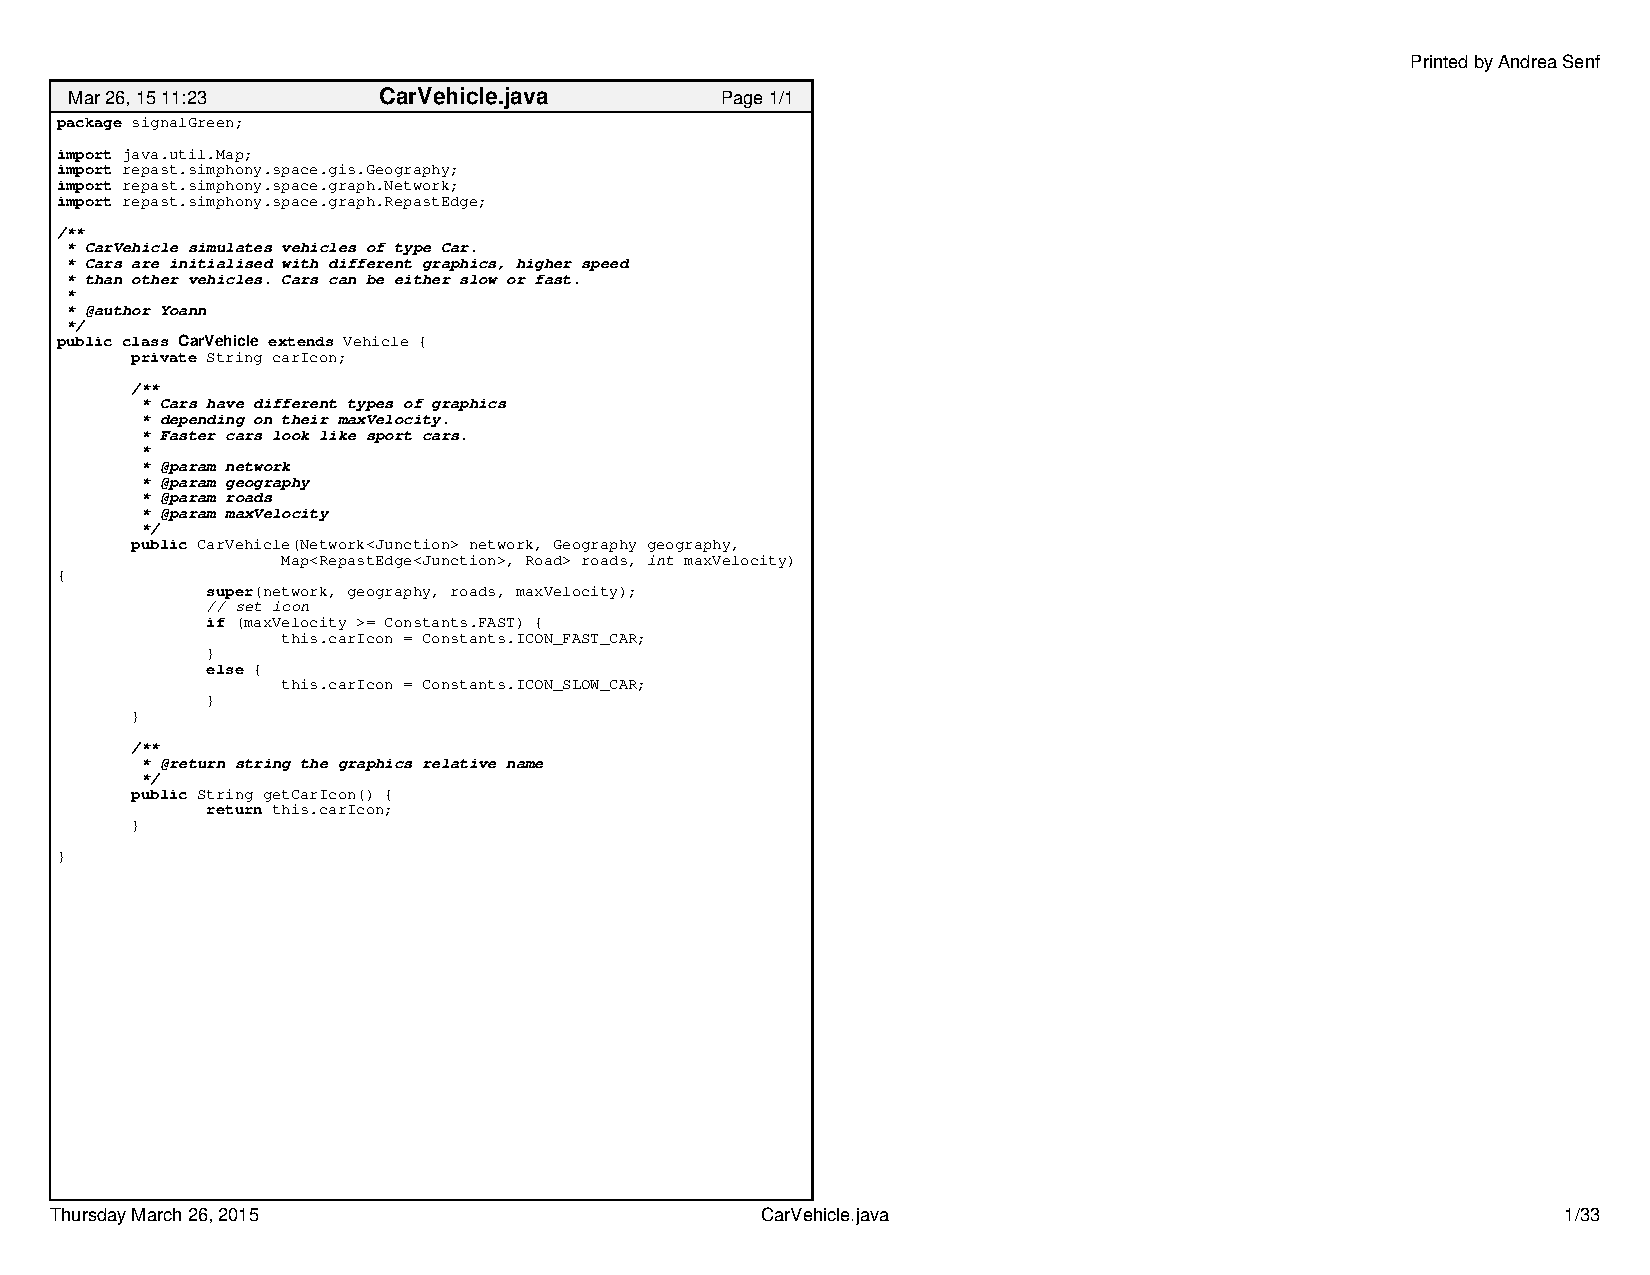
\includepdf[pages={1-}]{sourcecode.pdf}


\end{appendices}




\end{document}



